% Интро
Большие языковые модели (large language models, LLMs), типа GPT \cite{gpt2, gpt3}, способны достаточно хорошо изучить распределение своего обучающего набора данных, чтобы затем генерировать реалистичный текст.
При обучении большой языковой модели используется огромный набор данных, собранный по всему интернету, в котором содержатся тексты различного содержания и различных стилей.
Поэтому имеет смысл пытаться управлять генерацией языковой модели, чтобы результирующий текст имел желательную стилевую окраску.

% Суть
В работах \textit{GeDi: Generative Discriminator Guided
Sequence Generation} \cite{krause2020gedi} и \textit{Text Detoxification using Large Pre-trained Neural Models} \cite{dale2021text} предлагается управлять генерацией текста с помощью другой языковой модели, которая обучена на требуемом домене данных.

Предлагаемая модель GeDi состоит из двух компонент:
генеративная модель на основе GPT-2 и дискриминативная модель, тоже на основе GPT-2, но обученная с дополнительными метками стиля на уровне предложений.
Это заставляет модель дискриминатора выучивать распределения слов, обусловленные конкретным стилем.
На каждом шаге генерации, распределение токенов, полученное из основной модели $P_{LM}$ редактируется с помощью модели дискриминатора $P_D$ и правила Байеса:
$$
P(x_t|x_{<t},c) \propto P_{LM}(x_t|x_{<t})P_D(c|x_t,x_{<t})
$$
где $x_t$ это текущий токен, $x_{<t}$ уже сгенерированный текст, а $c$ это желаемый стилистический атрибут (один из $C$ классов).
Первый член генерируется основной языковой моделью $P_{LM}$, а второй вычисляется с помощью правила Байеса и дополнительной условной языковой модели $P_{CC}$.
Таким образом, токены, которые более вероятно окажутся в тексте желаемым стилем, получают более высокую вероятность:
$$
P_D(c|x_t, x_{<t}) \propto P(c)P_{CC}(x,x_{<t}|c)
$$
Принцип работы проиллюстрирован на рисунке \ref{fig:gedi_original}.
\begin{figure}[ht]
  \centering
  \frame{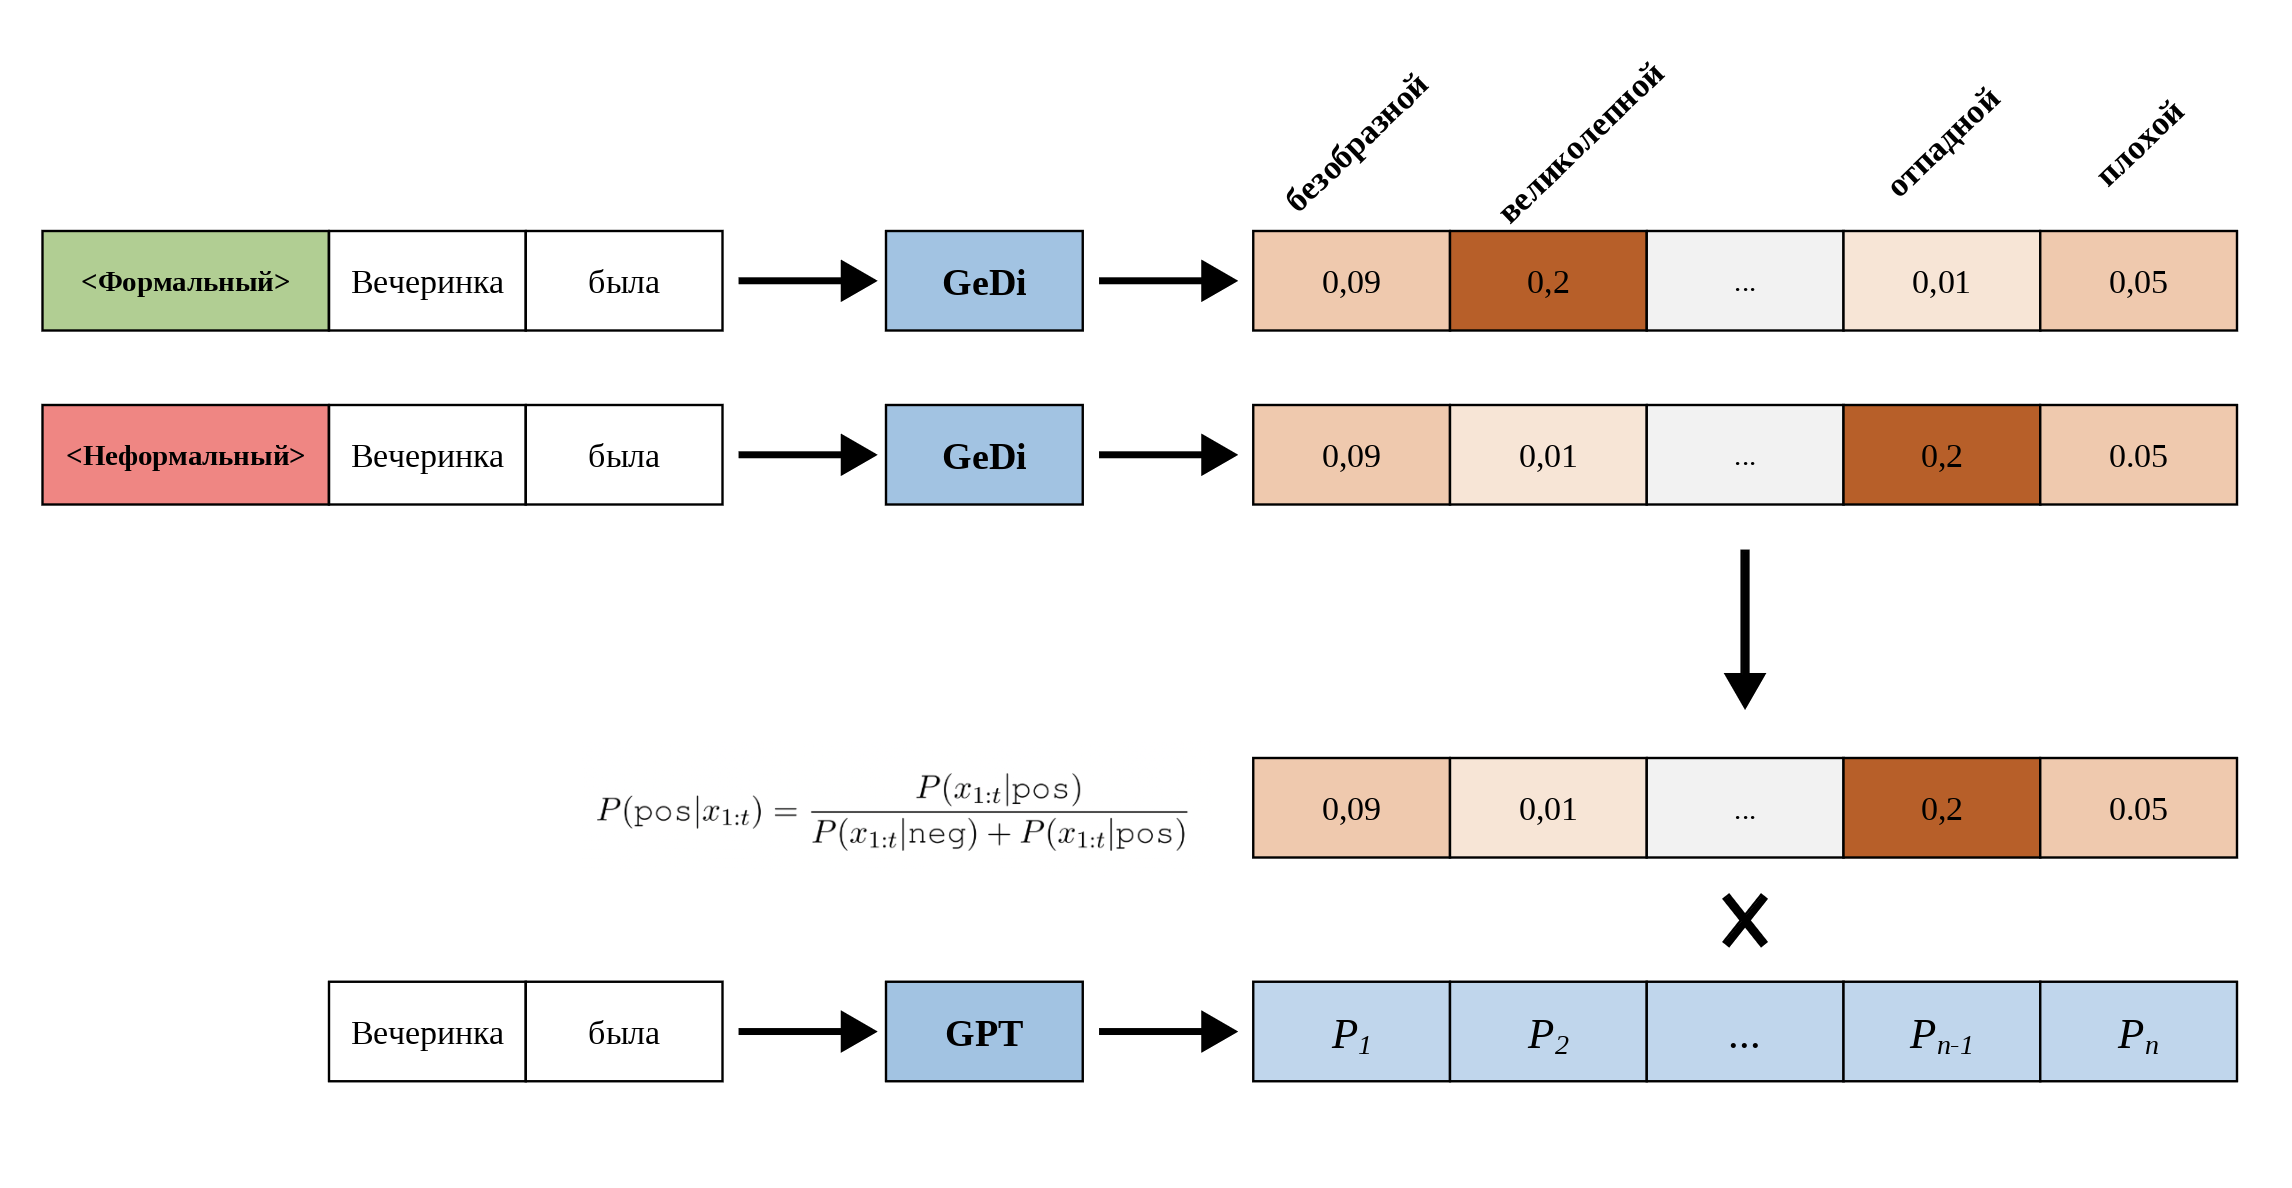
\includegraphics[width=1.0\textwidth]{figures/gedi_original.png}}
  \caption{Модель GeDi}
  \label{fig:gedi_original}
\end{figure}

Чтобы сохранить содержание предложения в работе \cite{dale2021text} предлагается заменить основную языковую модель на модель, обученную на генерацию парафраза.
Пусть $x$ это исходное предложение, $T$ длинна сгенерированного текста $y$, а $c$ это желаемый стиль, то предлагаемая модель моделирует следующую вероятность:
$$
P(y_t|y_{<t},x,x) \propto P_{LM}(y_t|y_{<t}, x)P(c|y_t,y_{<t},x)
\approx P_{LM}(y_t|y_{<t},x)P_D(c|y_t,y_{<t})
$$

Последнее это аппроксимация, потому что вероятность класса должна быть обусловленна как $x$, так и $y$.
Однако это приближение, хотя и не является полностью оправданным, позволяет     отделить модель парафраза (которая требует параллельного корпуса для обучения) от модели стиля (которая требует только текстов с метками стиля, не обязательно параллельных).
Общий принцип работы изображен на рисунке \ref{fig:gedi_paragedi}
\begin{figure}[ht]
  \centering
  \frame{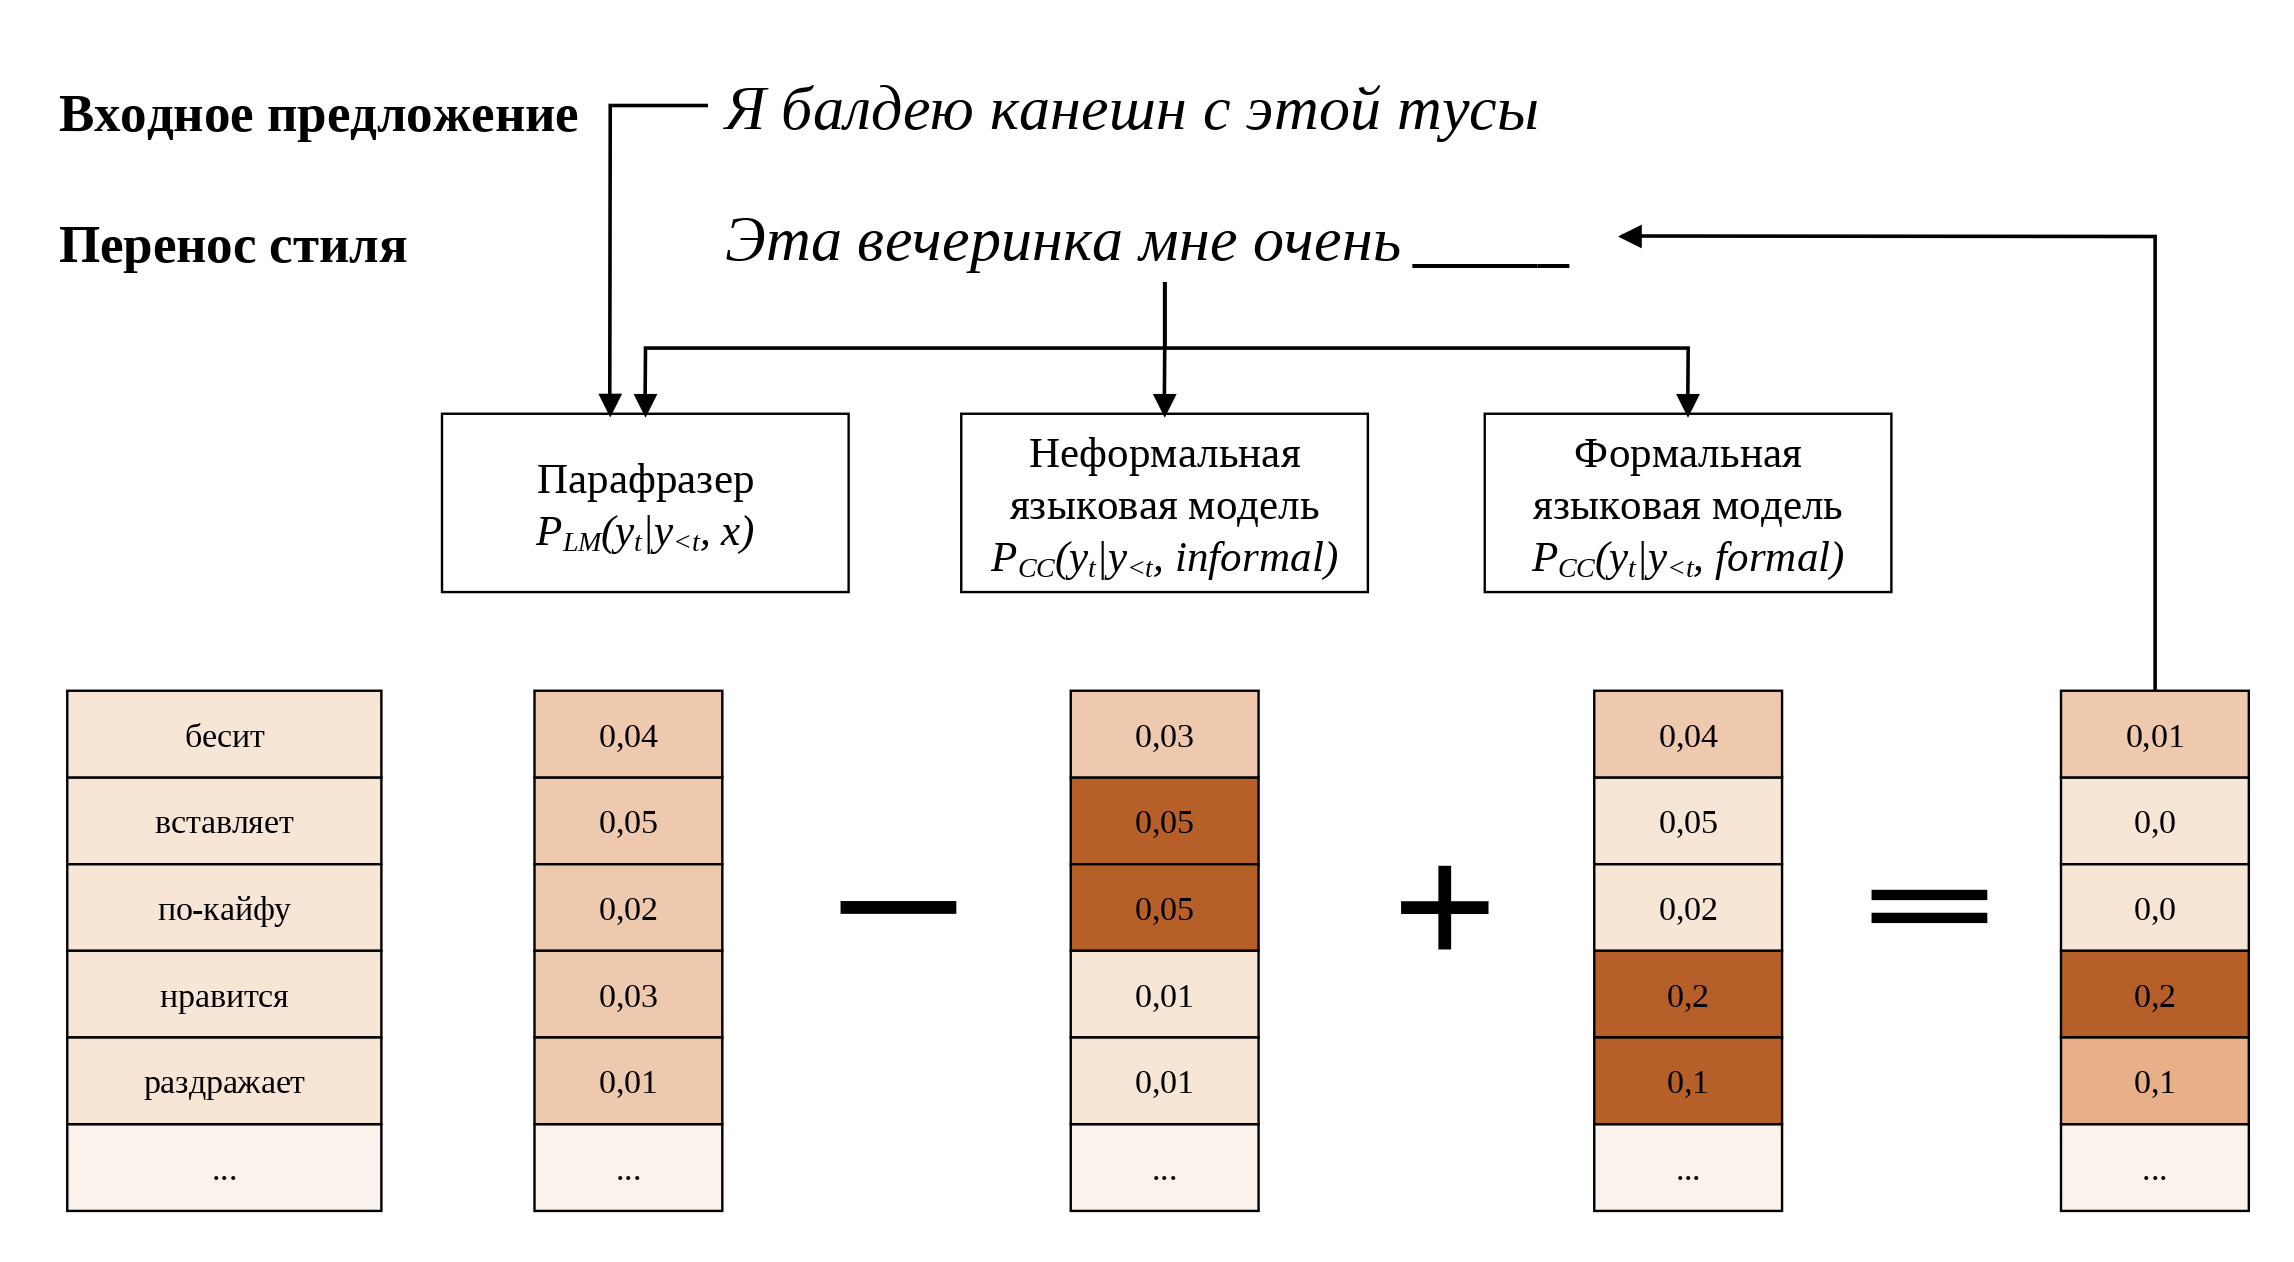
\includegraphics[width=1.0\textwidth]{figures/gedi_detox.png}}
  \caption{Использование модели парафразера в GeDi}
  \label{fig:gedi_paragedi}
\end{figure}

% Обучение
Функция потерь $\mathcal{L}_{ParaGeDi}$ состоит из линейной комбинации двух других функций потерь: генеративной $\mathcal{L}_G$, используемого в обучении языковой модели, и дискриминативной $\mathcal{L}_D$, которая отдаляет разные классы друг от друга в латентном пространстве.
$$
\mathcal{L}_G = - \frac{1}{N} \sum_{i=1}^N 
\frac{1}{T_i} \sum_{t=1}^{T_i} \log P (y_t^{(i)}|y_{<t}^{(i)}, c^{(i)})
$$
$$
\mathcal{L}_D = - \frac{1}{N} \sum_{i=1}^N \log P(c^{(i)}|y_{1:T_i}^{(i)})
$$
$$
\mathcal{L}_{ParaGeDi} = \lambda \mathcal{L}_D + (1 - \lambda) \mathcal{L}_G
$$

В качестве условной языковой модели была использована \texttt{ai-forever/rugpt3large\_based\_on\_gpt2}, а в качестве модели парафраза был взят предобученный \texttt{cointegrated/rut5-base-paraphraser}.

% Результаты и примеры
Метрики качества итогового алгоритма представлены в таблице \ref{table:results}, а примеры генерации в приложении \ref{cha:appendix1}.


% Можно заметить, что задача по переводу из неформального в формальный стиль также оказалась трудновыполнимой, но по сравнению с предыдущим методом был получен прирост в 0,12 по переводу в формальный стиль.

Заметим, что основаные на референсах n-грамные метрики значительно ухудшились, но в то же время можно наблюдать вполне удовлетворительные парафразы.
Здесь стоит сделать вывод и подтвердить другие недавние исследования \cite{li2018delete, mir2019evaluating, shen2022evaluation} о том, что несмотря на наличие параллельного набора данных данные метрики для этой задачи являются не самыми адекватными.
Ведь каждый конкретный стиль может быть выражен разными конструкциями и нет однозначного сопоставления.



